\section{図の挿入}\label{sec:no2}

platexとdvipdfmxを組み合わせていた時は,extrabbコマンドなどでbbファイルを作ってやる必要があったが,最近は勝手にやってくれるようになった.

画像までのパスを入力するだけで
\begin{enumerate}
 \item \autoref{fig:nowprinting}のようにpdf
 \item \autoref{fig:nowprinting_png}のようにpng
 \item \autoref{fig:normal_distribution}のようにeps
 \item \autoref{fig:normal_distribution_jpg}のようにjpg
\end{enumerate}
を埋め込むことが可能.
拡大してみるとベクター形式かどうかで綺麗さが変わることが分かる.

\begin{figure}[htbp]
  \centering
  \begin{minipage}[b]{0.3\columnwidth}
    \centering
    \includegraphics[width=\columnwidth]{figs/nowprinting}
    \subcaption{pdfの参考例}
    \label{fig:nowprinting}
  \end{minipage}
  \begin{minipage}[b]{0.3\columnwidth}
    \centering
    \includegraphics[width=\columnwidth]{figs/nowprinting_png}
    \subcaption{pngの参考例2}
    \label{fig:nowprinting_png}
  \end{minipage}
  \\
  \begin{minipage}[b]{0.4\columnwidth}
    \centering
    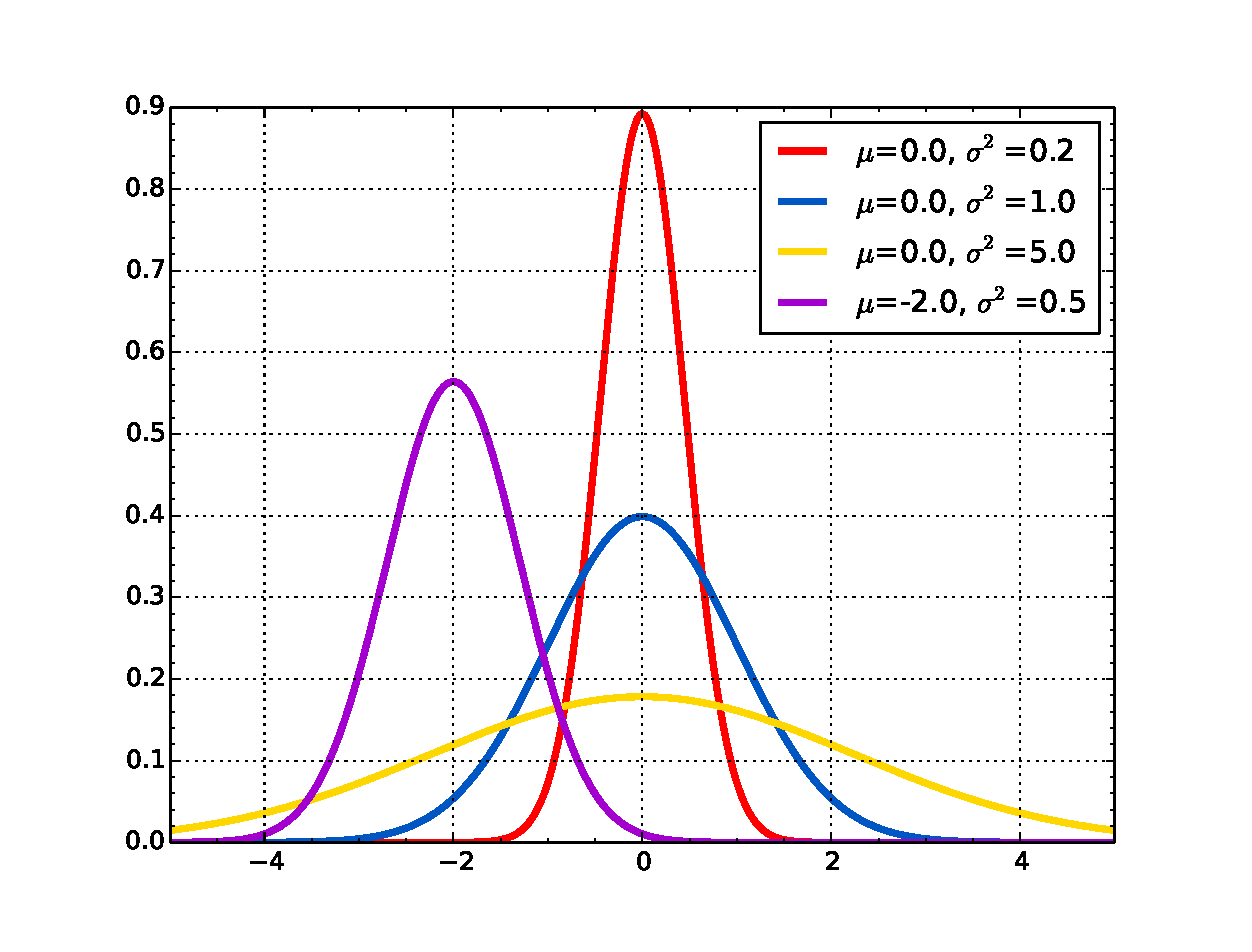
\includegraphics[width=\columnwidth]{figs/normal_distribution}
    \subcaption{epsの参考例}
    \label{fig:normal_distribution}
  \end{minipage}
  \begin{minipage}[b]{0.4\columnwidth}
    \centering
    \includegraphics[width=\columnwidth]{figs/normal_distribution_jpg}
    \subcaption{jpgの参考例}
    \label{fig:normal_distribution_jpg}
  \end{minipage}
  \caption{図の参考例}
  \label{fig:example-of-figures}
\end{figure}

\autoref{listing:normal_distribution}のようにlistingを使えばソースコードを貼ることも可能.
こちらもパスを指定してあげるだけでOK.
本当はlistingではなくてmintedを使いたいが,pdflatexでないとmintedは使えないようなので,残念ポイント.

\lstinputlisting[language=Python, caption=normal\_distribution.py, label=listing:normal_distribution, numbers=left, showstringspaces=false,
  keywordstyle={\bfseries \color[cmyk]{1,0,0.1,0}},
  stringstyle={\ttfamily \color[cmyk]{0.5,0,1,0}},
  basicstyle=\ttfamily\small]{codes/normal_distribution.py}
